\chapter{Specific Requirements}
This section is devoted to a specific description of every kind of requirement the
system has to deal with in order to achieve all the functionalities described.
\section{External interface Requirements}
\subsection{User Interfaces}
The mobile app is the interface which permit customers to enjoy CLup services. Whether installed on a smartphone or on a ticketing kiosk, it is the only way
for a customer to use CLup.
User interface mockups of most important pages of the app are shown below.

\vspace{0.5cm}
\begin{minipage}{.5\textwidth}
	\centering
	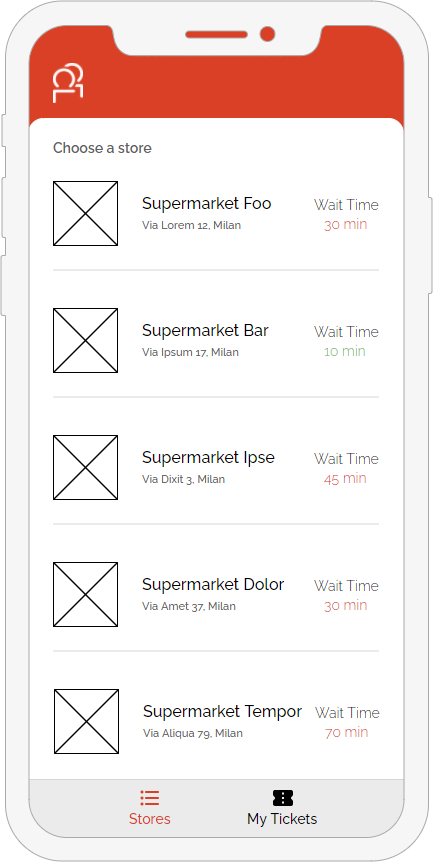
\includegraphics[scale=0.8]{home}
	\captionsetup{type=figure}
	\caption{App home.}
\end{minipage}%
\begin{minipage}{.5\textwidth}
	\centering
	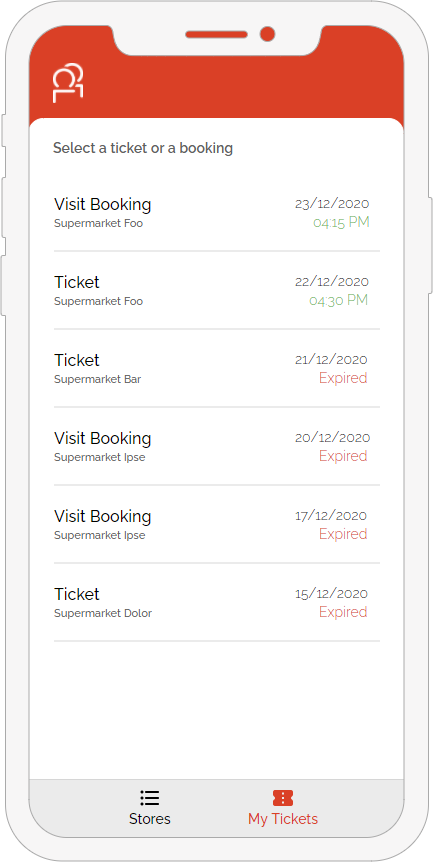
\includegraphics[scale=0.8]{my_tickets}
	\captionsetup{type=figure}
	\caption{Tickets list.}
\end{minipage}

\clearpage

\begin{minipage}{.5\textwidth}
	\centering
	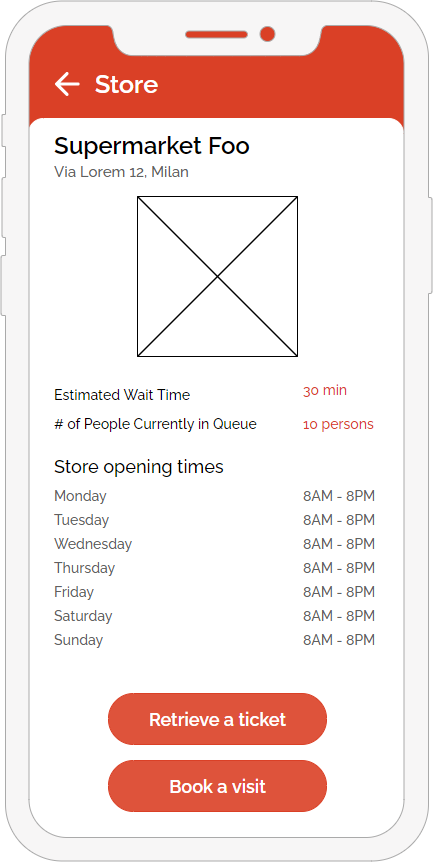
\includegraphics[scale=0.8]{store}
	\captionsetup{type=figure}
	\caption{Store page.}
\end{minipage}%
\begin{minipage}{.5\textwidth}
	\centering
	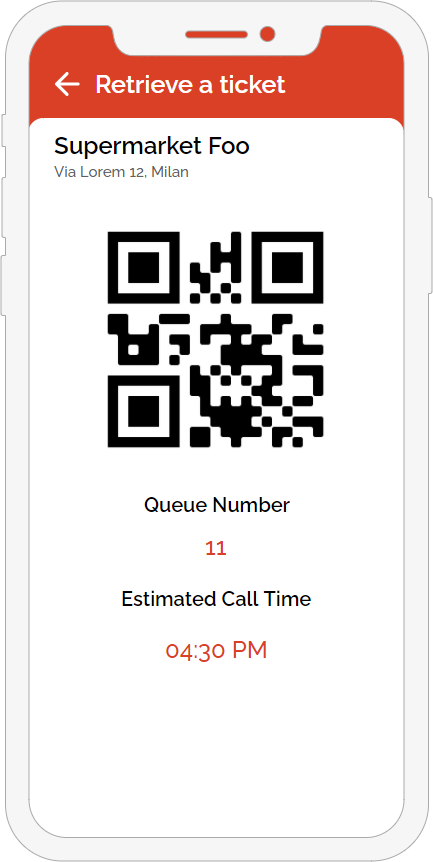
\includegraphics[scale=0.8]{ticket}
	\captionsetup{type=figure}
	\caption{Ticket Retrieved.}
\end{minipage}

\vspace{1cm}

\begin{minipage}{.5\textwidth}
	\centering
	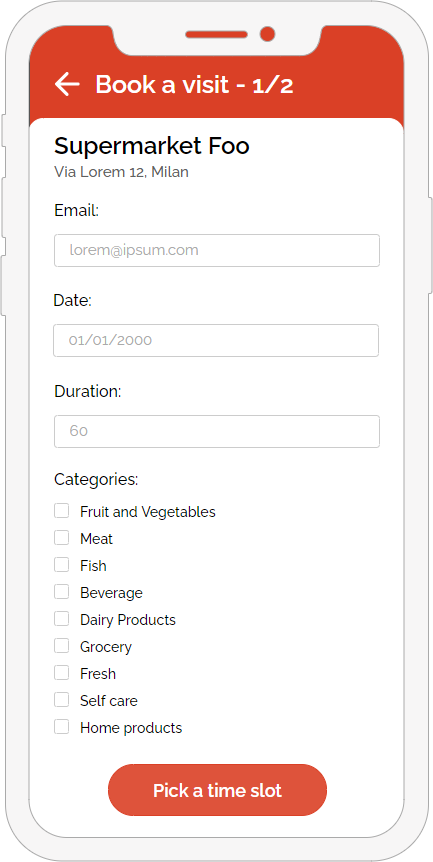
\includegraphics[scale=0.8]{book1}
	\captionsetup{type=figure}
	\caption{Book a visit (1/2).}
\end{minipage}%
\begin{minipage}{.5\textwidth}
	\centering
	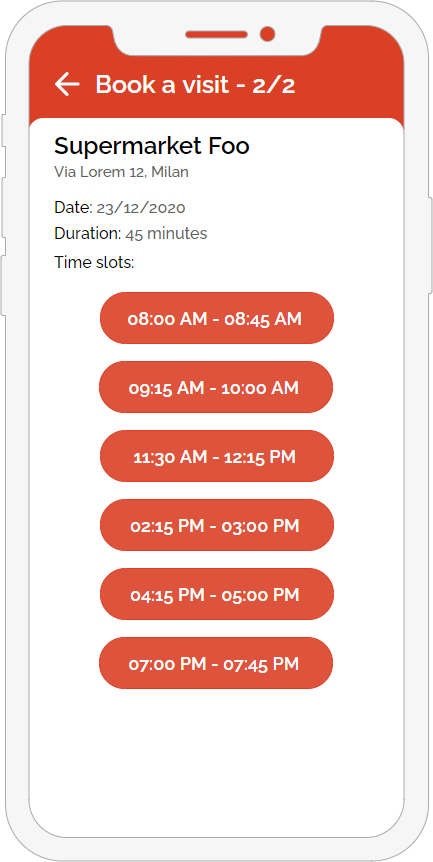
\includegraphics[scale=0.8]{book2}
	\captionsetup{type=figure}
	\caption{Book a visit (2/2).}
\end{minipage}

\vspace{1cm}

\begin{figure}[H]
	\centering
	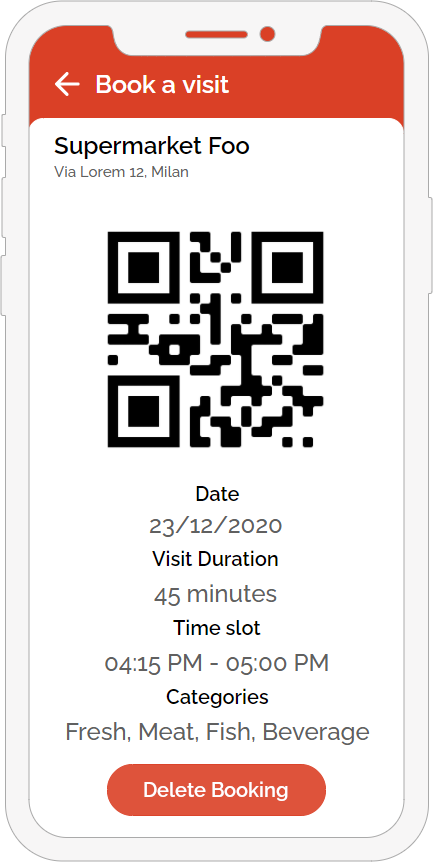
\includegraphics[scale=0.8]{book3}
	\caption{Visit booked.}
\end{figure}

\clearpage

Store managers and store employees use a web based interface for enjoying CLup features. The CLup admins can login at the same interface as well.
User interface mockups of most important pages of the web dashboard are shown below.
\vspace{0.5cm}
\begin{figure}[H]
	\centering
	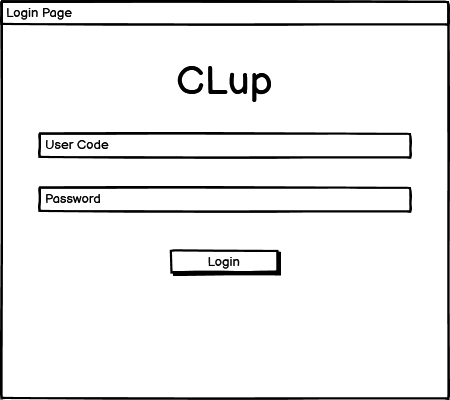
\includegraphics[width=0.64\linewidth]{login}
	\caption{Dashboard login.}
\end{figure}
\begin{figure}[H]
	\centering
	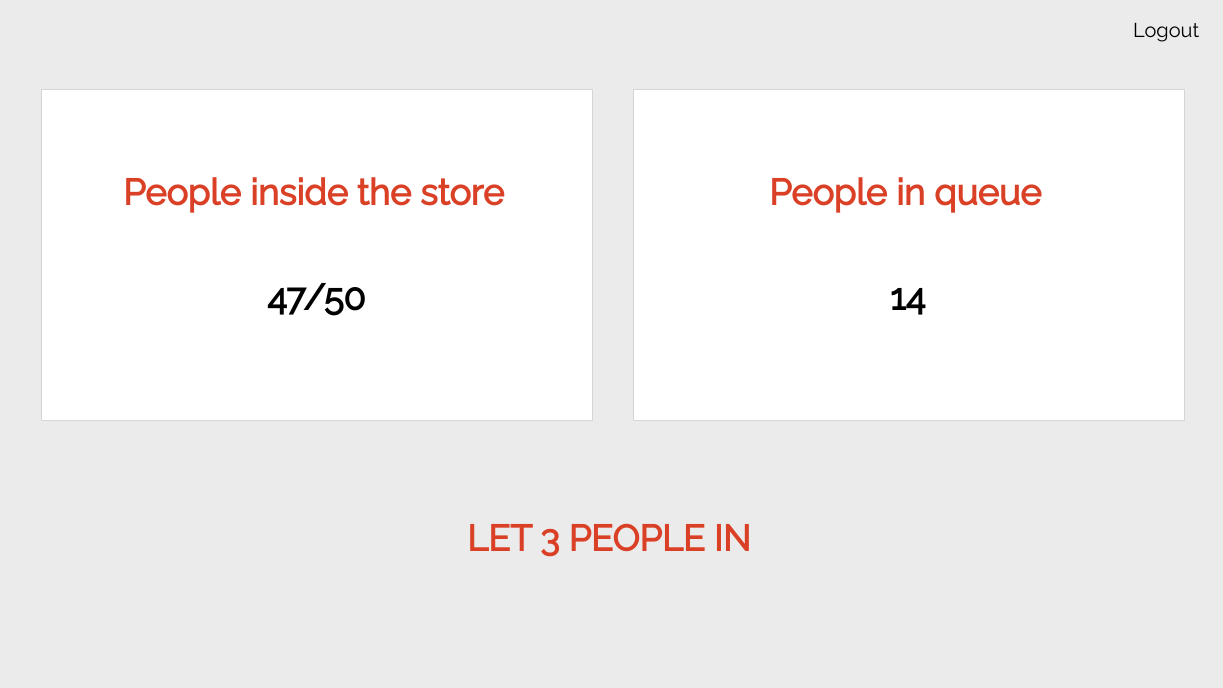
\includegraphics[width=0.64\linewidth]{employee}
	\caption{Employee homepage.}
\end{figure}
\begin{figure}[H]
	\centering
	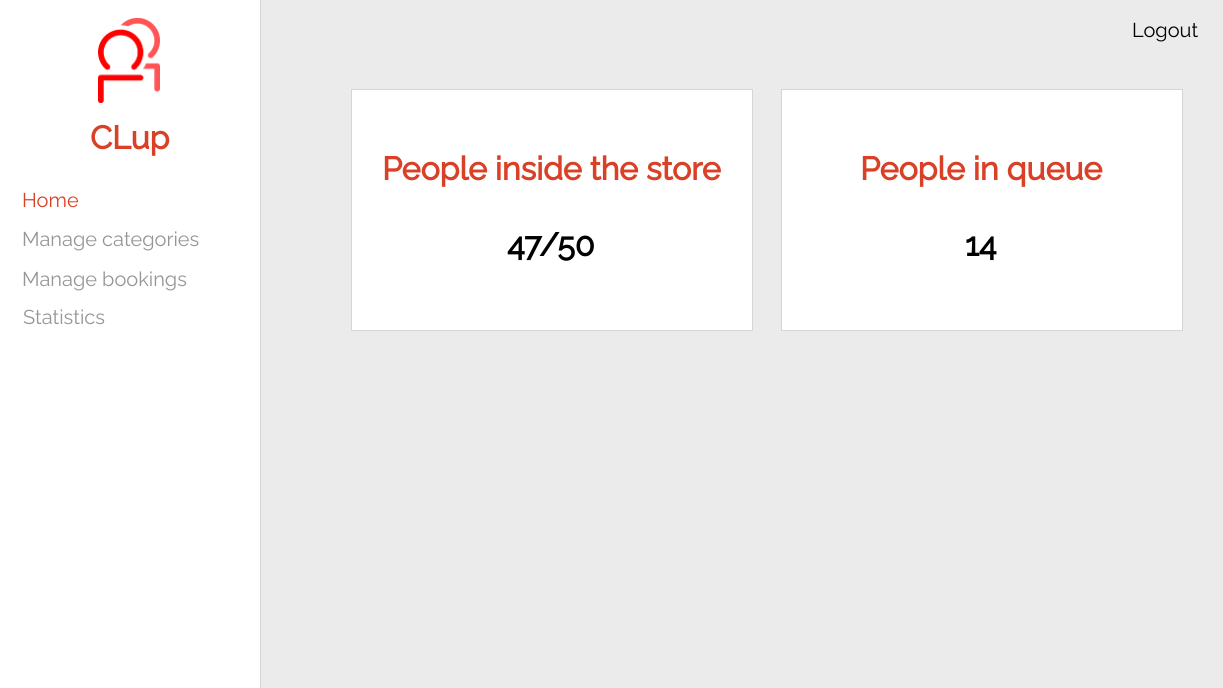
\includegraphics[width=0.64\linewidth]{dashboard1}
	\caption{Manager homepage.}
\end{figure}
\begin{figure}[H]
	\centering
	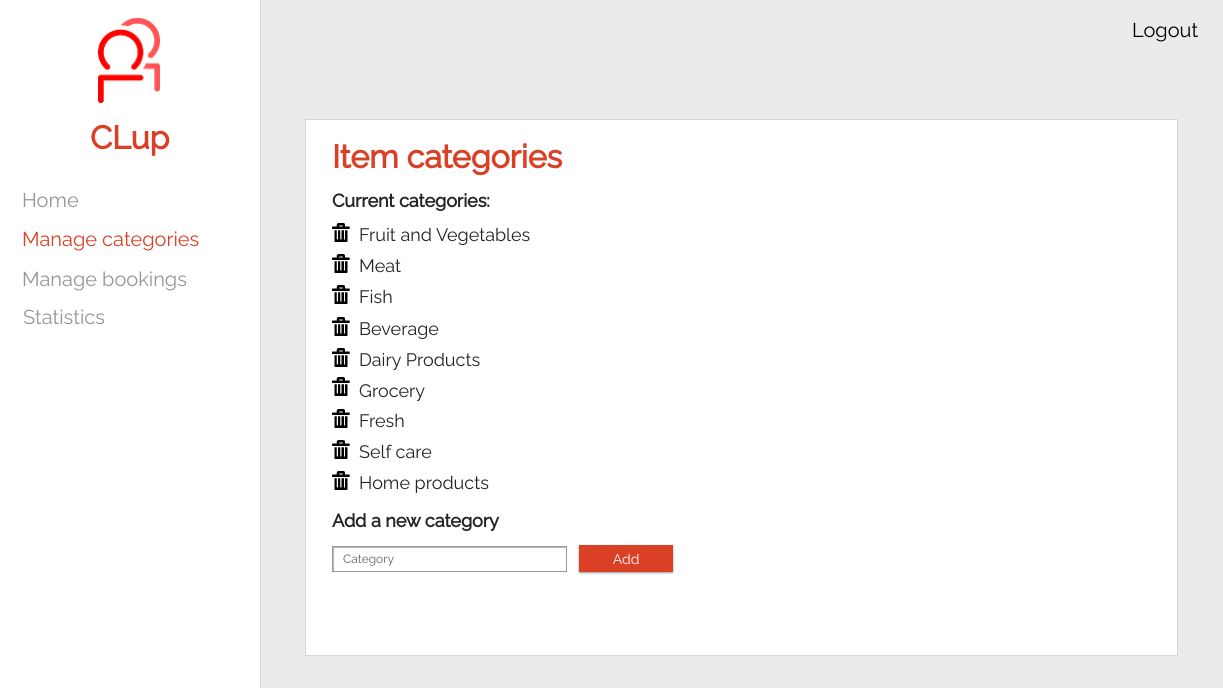
\includegraphics[width=0.64\linewidth]{dashboard2}
	\caption{Item categories page.}
\end{figure}
\begin{figure}[H]
	\centering
	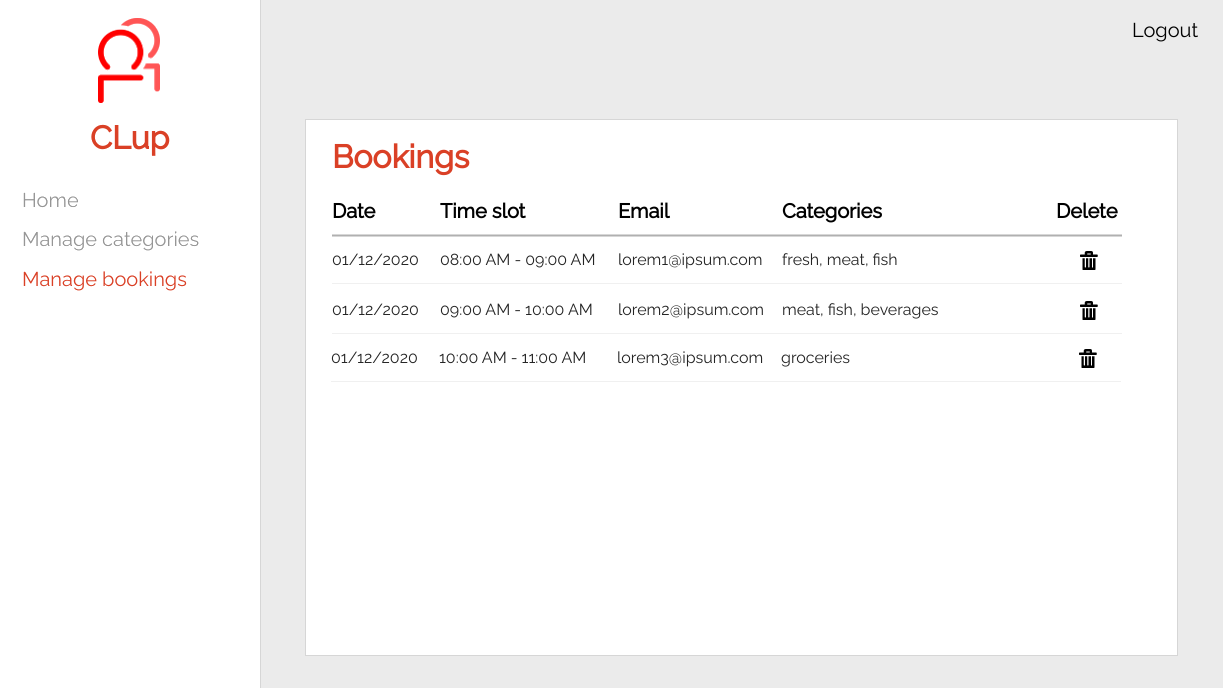
\includegraphics[width=0.64\linewidth]{dashboard3}
	\caption{Bookings list page.}
\end{figure}
\begin{figure}[H]
	\centering
	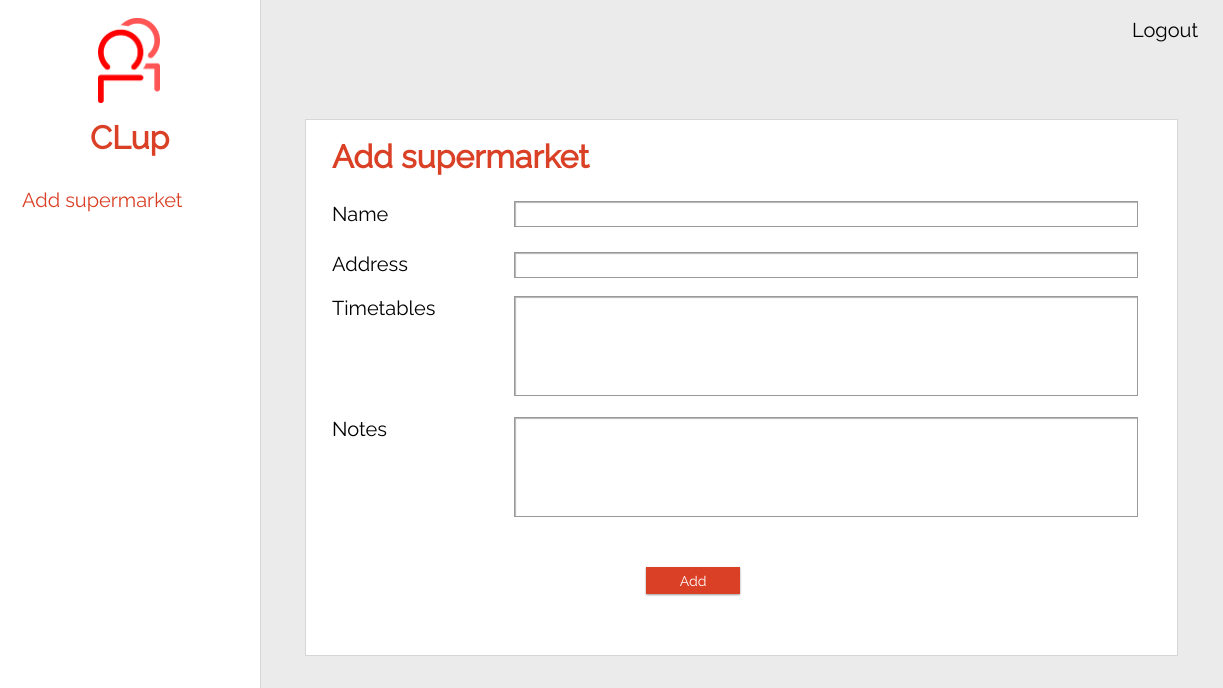
\includegraphics[width=0.64\linewidth]{new_store}
	\caption{Admin new supermarket page.}
\end{figure}

\clearpage

\subsection{Hardware Interfaces}
In addition to interfacing with computers (via a web browser), Clup interfaces with smartphones and their GPS module.
\subsection{Software Interfaces}
The system interfaces with a external map API for computing the distance between current place and store. It also permit to receive data
about QR codes via the public API.
\subsection{Communication Interfaces}
All the communications from and to CLup are made via HTTPS.

\section{Functional Requirements}
In this section, it is given a complete description of the functional requirements of the system.

    \subsection{Requirements}
    \subsubsection{Customer}
        \begin{enumerate}[series=requirements, label=\textbf{R.\arabic*}, leftmargin=+.3in]
            \item \itemtext{req:custQueue}{The system shall allow customers to line-up remotely in a store queue.}
            \item \itemtext{req:custTicket}{The system shall generate a new ticket when a customer enters a queue.}
            \item \itemtext{req:custTicketKiosk}{The system shall allow customers which do not have a smartphone to get a ticket in place.}
            \item \itemtext{req:custNum}{The system shall allow customers to view the number of people lined up in a queue.}
            \item \itemtext{req:custTime}{The system shall give customers an estimated waiting time.}
            \item \itemtext{req:custGps}{The system shall retrieve the GPS position while the user is subscribed to a queue.}
            \item \itemtext{req:custLeave}{The system shall allow customers to leave a queue.}
            \item \itemtext{req:custFilter}{The system shall allow customers to filter stores by name.}
            \item \itemtext{req:custTtl}{The system shall notify customers when it's time to leave for the store.}
            \item \itemtext{req:custBook}{The system shall allow customers to book-a-visit to the store and send them the confirmation link and receipt via email.}
            \item \itemtext{req:custItems}{The system shall allow book-a-visit customers to specify the main categories of item they intend to buy.}
            \item \itemtext{req:custDelete}{The system shall allow customers to delete a booked visit.}
            \item \itemtext{req:custNotifyDelete}{The system shall notify customers when a ticket or booked visit is deleted.}
        \end{enumerate}

    \subsubsection{Store manager}
    \begin{enumerate}[resume*=requirements]
        \item \itemtext{req:mngLogin}{A registered store manager must be able to login to the system by using their credentials.}
        \item \itemtext{req:mngViewStore}{The system shall allow store managers to view the current status of people inside the store.}
        \item \itemtext{req:mngViewQueue}{The system shall allow store managers to view the current status of people in the queue.}
         \item \itemtext{req:mngViewBook}{The system shall allow store managers to view the booked visits to the store.}
        \item \itemtext{req:mngCapStore}{The system shall allow store managers to set a maximum cap of people inside the store.}
        \item \itemtext{req:mngDeleteTickets}{The system shall allow store managers to delete tickets and booked visits.}
    \end{enumerate}

    \subsubsection{Store staff}
    \begin{enumerate}[resume*=requirements]
        \item \itemtext{req:stfLogin}{A registered store staff must be able to login to the system by using their credentials.}
        \item \itemtext{req:stfViewStore}{The system shall allow store staff to view the current status of people inside the store.}
        \item \itemtext{req:stfViewQueue}{The system shall allow store staff to view the current status of people in the queue.}
    \end{enumerate}

    \subsubsection{CLup admin}
    \begin{enumerate}[resume*=requirements]
        \item \itemtext{req:admRegister}{The system shall allow CLup admins to register new supermarkets.}
        \item \itemtext{req:admCredentials}{The system shall generate new manager and staff credential for each supermarket registered.}
    \end{enumerate}

    \subsection{Goal mapping on requirements}

    \begin{description}


        \item \printitem{goal:avoidQueue}

        \begin{description}

        	\item \printitem{goal:custHazardSit}

			\printitem{req:custQueue}
			\printitem{req:custNum}
			\printitem{req:custTime}
			\printitem{req:custTtl}
			\printitem{req:custBook}
			\printitem{req:custItems}

			\printitem{dom:smartphone}
			\printitem{dom:categories}
			\printitem{dom:custEmail}
			\printitem{dom:oneToOneQr}
			\printitem{dom:timeArrival}


			\item \printitem{goal:storeHazardSit}

			\printitem{req:mngViewStore}
			\printitem{req:mngViewQueue}
			\printitem{req:mngViewBook}
			\printitem{req:mngCapStore}
			\printitem{req:mngDeleteTickets}
			\printitem{req:stfViewStore}
			\printitem{req:stfViewQueue}

			\printitem{dom:categories}
			\printitem{dom:oneToOneQr}
			\printitem{dom:internetStores}
			\printitem{dom:pecStores}
			\printitem{dom:employeeEntrance}
			\printitem{dom:timeArrival}
			\printitem{dom:capStores}


            \item \printitem{goal:shortenTime}

           	\printitem{req:custQueue}
           	\printitem{req:custNum}
           	\printitem{req:custTime}
           	\printitem{req:custTtl}
           	\printitem{req:custBook}

           	\printitem{dom:smartphone}
           	\printitem{dom:workingGps}
           	\printitem{dom:gpsPrecision}
           	\printitem{dom:bringSmartphone}
           	\printitem{dom:employeeEntrance}
           	\printitem{dom:qrServiceReliable}
           	\printitem{dom:qrServiceApi}
           	\printitem{dom:timeArrival}


            \item \printitem{goal:arriveOnTime}

           	\printitem{req:custQueue}
           	\printitem{req:custNum}
           	\printitem{req:custTime}
           	\printitem{req:custGps}
           	\printitem{req:custTtl}
           	\printitem{req:custBook}

           	\printitem{dom:smartphone}
           	\printitem{dom:workingGps}
           	\printitem{dom:gpsPrecision}
           	\printitem{dom:bringSmartphone}
           	\printitem{dom:timeArrival}
		\end{description}

        \item \printitem{goal:otherTasks}

       	\printitem{req:custQueue}
       	\printitem{req:custNum}
       	\printitem{req:custTime}
       	\printitem{req:custTtl}
       	\printitem{req:custBook}

       	\printitem{dom:smartphone}
       	\printitem{dom:workingGps}
       	\printitem{dom:gpsPrecision}
       	\printitem{dom:custEmail}
       	\printitem{dom:bringSmartphone}
       	\printitem{dom:timeArrival}


        \item \printitem{goal:easyExp}

       	\printitem{req:custTicket}
       	\printitem{req:custNum}
       	\printitem{req:custTime}
       	\printitem{req:custLeave}
       	\printitem{req:custFilter}
       	\printitem{req:custBook}
       	\printitem{req:custDelete}
       	\printitem{req:custNotifyDelete}

       	\printitem{dom:smartphone}
       	\printitem{dom:workingGps}
       	\printitem{dom:uniqueName}
       	\printitem{dom:qrServiceReliable}
       	\printitem{dom:storeRegistered}
       	\printitem{dom:storeKiosk}


        \item \printitem{goal:enjoyService}

       	\printitem{req:custQueue}
       	\printitem{req:custTicketKiosk}
       	\printitem{req:custBook}

       	\printitem{dom:smartphone}
       	\printitem{dom:internetStores}
       	\printitem{dom:pecStores}
       	\printitem{dom:storeRegistered}
       	\printitem{dom:storeKiosk}


        \item \printitem{goal:monitorAccess}

       	\printitem{req:mngLogin}
       	\printitem{req:mngViewStore}
       	\printitem{req:mngViewQueue}
       	\printitem{req:mngViewBook}
       	\printitem{req:stfLogin}
       	\printitem{req:stfViewStore}
       	\printitem{req:stfViewQueue}
       	\printitem{req:admRegister}
       	\printitem{req:admCredentials}

       	\printitem{dom:internetStores}
       	\printitem{dom:pecStores}
       	\printitem{dom:employeeEntrance}
       	\printitem{dom:storeRegistered}
       	\printitem{dom:capStores}


        \item \printitem{goal:knowInAdvance}

       	\printitem{req:mngViewStore}
       	\printitem{req:mngViewQueue}
       	\printitem{req:mngViewBook}
       	\printitem{req:stfViewStore}
       	\printitem{req:stfViewQueue}

       	\printitem{dom:smartphone}
       	\printitem{dom:categories}
       	\printitem{dom:internetStores}
       	\printitem{dom:pecStores}
       	\printitem{dom:storeRegistered}


        \item \printitem{goal:limitNumber}

       	\printitem{req:mngCapStore}
       	\printitem{req:mngDeleteTickets}

       	\printitem{dom:smartphone}
       	\printitem{dom:categories}
       	\printitem{dom:internetStores}
       	\printitem{dom:pecStores}
       	\printitem{dom:storeRegistered}
       	\printitem{dom:timeArrival}
       	\printitem{dom:capStores}

    \end{description}

	\clearpage
    \subsection{Scenarios}
		\subsubsection{Scenario 1}
		John has to go to the supermarket to buy some groceries. Since there is a pandemic going on, he would like to go there as safely as possible.\newline
		So he opens CLup, chooses his trusted supermarket and takes a queue ticket. The application tells him to go to the supermarket at 12:30 and since John is about ten minutes away from the store it notifies him to leave at 12:20. Once in the store an employee checks the ticket by scanning his QR code and John can enter the supermarket.
		At the exit the cashier will scan again the QR to notify the exit of a customer from the store.
		\subsubsection{Scenario 2}
		Tomorrow John is going to go for work near the largest Essecorta in the province. There is no better opportunity to go shopping in his favourite supermarket.\newline
		However, since he will be tight on time, he needs to book a visit to the store so he won't lose even a minute. Thus, he takes his phone and opens CLup, he chooses the store from the list and enters some informations, like the category of items he would like to buy. He adds the desired time slot and finally opens the email that just arrived and confirms his booking: he is now ready to go.
		\subsubsection{Scenario 3}
		John's business appointment near the famous Essecorta has been cancelled. For this reason, he can no longer go to the store.\newline
		Since John is a model citizen, he decides to delete the booking that he did with CLup. So he opens the app, he goes to the store pass section and deletes the bookings.
		\subsubsection{Scenario 4}
		The CLup admin Bob was contacted from the manager of Superal store near the Cathedral to provide CLup to his customers. After asking him some informations about the store, like Name and PEC, the admin fills the form for register a new store on the dashboard. From now on the customers of Superal can enjoy the service.
		\subsubsection{Scenario 5}
		The Superal store has recently expanded due to some renovation works. The manager Alice wants to increase the number of maximum customer inside the store and monitor them.\newline
		For doing so, she goes to the CLup dashboard, logs in and increases the maximum cap. From that page she also watches the number of customers inside the store.

	\clearpage
    \subsection{Use cases description}
    Use cases capture functional requirements of a system from the users' perspective.

	\begin{table}[H]
    	\centering
		\begin{tabular}{@{}p{0.25\linewidth}p{0.71\linewidth}@{}}
			\toprule
			\textbf{Name} & Retrieve ticket \\

			\midrule
			\textbf{ID} & \usecaseindex{uc:retrieveTicket} ~\\
			\midrule
			\textbf{Actors} & Customer \\
			\midrule
			\textbf{Entry conditions} &
				\begin{itemize}[leftmargin=.4cm,noitemsep,topsep=0pt,before=\vspace{-3mm},after=\vspace{-4mm}]
					\item The customer has installed the application on their device;
					\item The application is running.
				\end{itemize} \\
			\midrule
			\textbf{Flow of events} &
				\begin{enumerate}[label=\roman*.,leftmargin=.5cm,noitemsep,topsep=0pt,before=\vspace{-3mm},after=\vspace{-4mm}]
					\item The customer selects a store from the home page;
					\item The customer presses the "Retrieve Ticket" button.
                    \item If the GPS is enabled, the application notifies the customer when it's time to leave.
				\end{enumerate} \\
			\midrule
			\textbf{Exit conditions} & The customer has retrieved a ticket for the selected store. \\
			\midrule
			\textbf{Exceptions} &
                \begin{itemize}[leftmargin=.4cm,noitemsep,topsep=0pt,before=\vspace{-3mm},after=\vspace{-4mm}]
                    \item If the customer has already retrieved a ticket for a store, the system displays an error message telling the customer they cannot get more than one ticket simultaneously.
                    \item If the system fails to retrieve the GPS location, no notification will be shown.
                \end{itemize} \\
			\bottomrule
		\end{tabular}
		\caption{\textit{Retrieve ticket} use case description.}
	\end{table}

	\begin{figure}[H]
		\centering
		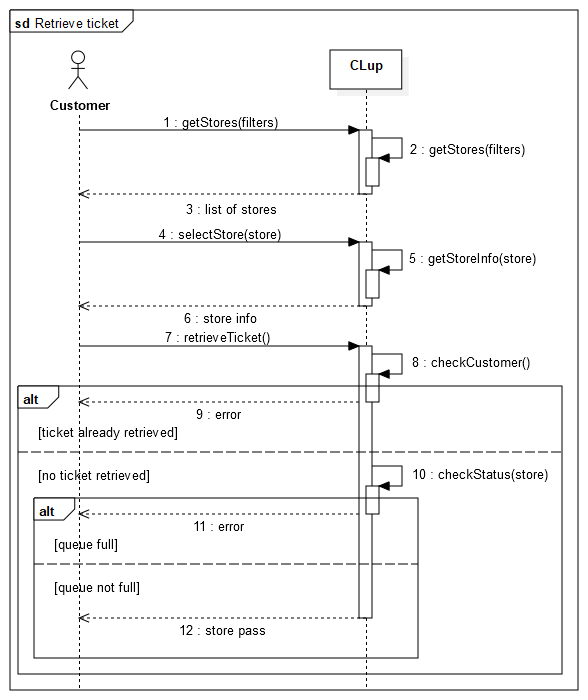
\includegraphics[width=\linewidth]{sd_retrieve_ticket}
		\caption{\textit{Retrieve ticket} sequence diagram.}
	\end{figure}

	\begin{table}[H]
    	\centering
    	\begin{tabular}{@{}p{0.25\linewidth}p{0.71\linewidth}@{}}
    		\toprule
    		\textbf{Name} & Book a visit \\

    		\midrule
    		\textbf{ID} & \usecaseindex{uc:bookVisit} ~\\
    		\midrule
    		\textbf{Actors} & Customer \\
    		\midrule
    		\textbf{Entry conditions} &
    		\begin{itemize}[leftmargin=.4cm,noitemsep,topsep=0pt,before=\vspace{-3mm},after=\vspace{-4mm}]
    			\item The customer has installed the application on their device;
    			\item The application is running.
    		\end{itemize} \\
    		\midrule
    		\textbf{Flow of events} &
    		\begin{enumerate}[label=\roman*.,leftmargin=.5cm,noitemsep,topsep=0pt,before=\vspace{-3mm},after=\vspace{-4mm}]
    			\item The customer selects a store from the home page;
    			\item The customer presses the "Book a visit" button;
    			\item The customer inserts their email address, the date, the approximate duration of the visit and the main categories of items they intend to buy;
    			\item The customer selects the time slot;
                \item The customer submits the form;
                \item The system shows to the customer the booked visit.
                \item If the GPS is enabled, the application notifies the customer when it's time to leave.
    		\end{enumerate} \\
    		\midrule
    		\textbf{Exit conditions} & The customer has retrieved a ticket for the selected store. \\
    		\midrule
    		\textbf{Exceptions} &
            \begin{itemize}[leftmargin=.4cm,noitemsep,topsep=0pt,before=\vspace{-3mm},after=\vspace{-4mm}]
                \item If the customer has already booked a visit to a store in a certain date, the system displays an error message telling the customer it cannot book again for the same day at the same store;
                \item If the customer selects a date so that there are no more available time slots, the system displays an error message telling the customer to select a different date.
                \item If the system fails to retrieve the GPS location, no notification will be shown.
            \end{itemize} \\

    		\bottomrule
    	\end{tabular}
    	\caption{\textit{Book a visit} use case description.}
    \end{table}

	\begin{figure}[H]
		\centering
		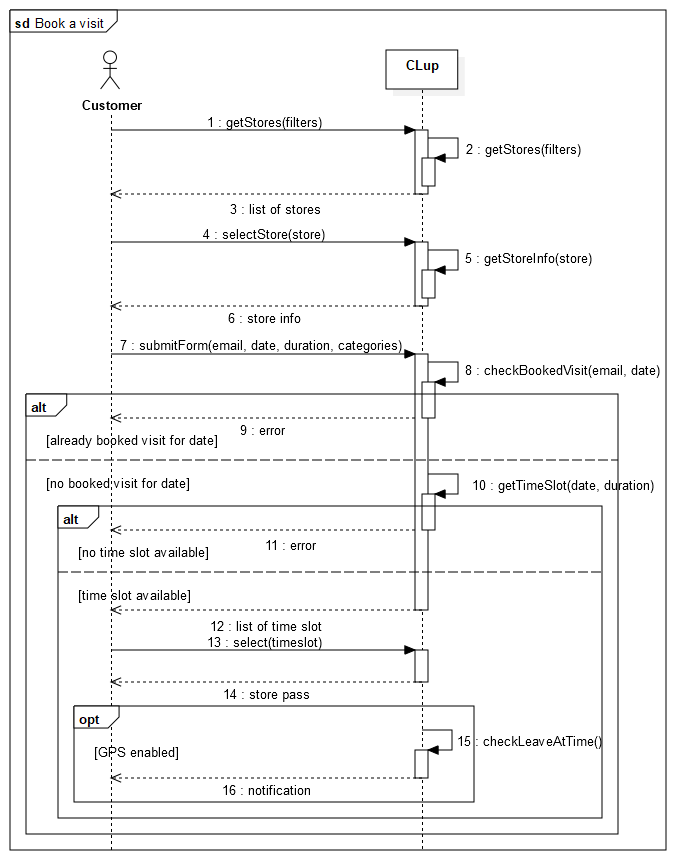
\includegraphics[width=\linewidth]{sd_book_a_visit}
		\caption{\textit{Book a visit} sequence diagram.}
	\end{figure}

	\begin{table}[H]
        \centering
        \begin{tabular}{@{}p{0.25\linewidth}p{0.71\linewidth}@{}}
            \toprule
            \textbf{Name} & Delete a store pass \\

            \midrule
            \textbf{ID} & \usecaseindex{uc:deletePass} ~\\
            \midrule
            \textbf{Actors} & Customer \\
            \midrule
            \textbf{Entry conditions} &
            \begin{itemize}[leftmargin=.4cm,noitemsep,topsep=0pt,before=\vspace{-3mm},after=\vspace{-4mm}]
                \item The customer has installed the application on their device;
                \item The application is running.
            \end{itemize} \\
            \midrule
            \textbf{Flow of events} &
            \begin{enumerate}[label=\roman*.,leftmargin=.5cm,noitemsep,topsep=0pt,before=\vspace{-3mm},after=\vspace{-4mm}]
                \item The customer swipes to the "My Store Pass" page;
                \item The customer selects one of the available store passes;
                \item The customer presses the "Delete Store Pass" button;
                \item The customer selects "Yes" on the confirmation message;
                \item The customer is notified by the system that the store pass has been deleted successfully.
            \end{enumerate} \\
            \midrule
            \textbf{Exit conditions} & The customer has deleted successfully a store pass. \\
            \midrule
            \textbf{Exceptions} & If the customer has no store pass, the system displays a label: "No store pass available". \\
            \bottomrule
        \end{tabular}
        \caption{\textit{Delete a store pass} use case description.}
    \end{table}

	\begin{figure}[H]
		\centering
		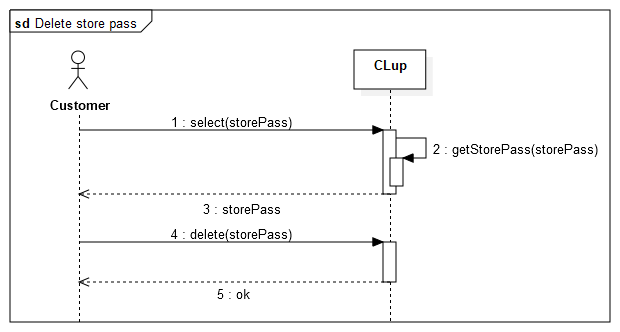
\includegraphics[width=\linewidth]{sd_delete_store_pass}
		\caption{\textit{Delete a store pass} sequence diagram.}
	\end{figure}


	\begin{table}[H]
        \centering
        \begin{tabular}{@{}p{0.25\linewidth}p{0.71\linewidth}@{}}
            \toprule
            \textbf{Name} & Web platform login \\

            \midrule
            \textbf{ID} & \usecaseindex{uc:webLogin} ~\\
            \midrule
            \textbf{Actors} & Store manager, Store employee, CLup admin \\
            \midrule
            \textbf{Entry conditions} &
            \begin{itemize}[leftmargin=.4cm,noitemsep,topsep=0pt,before=\vspace{-3mm},after=\vspace{-4mm}]
                \item The web platform is running.
            \end{itemize} \\
            \midrule
            \textbf{Flow of events} &
            \begin{enumerate}[label=\roman*.,leftmargin=.5cm,noitemsep,topsep=0pt,before=\vspace{-3mm},after=\vspace{-4mm}]
                \item The actor goes to the login page;
                \item The actor inserts their username and password;
                \item The actor submits the form.
            \end{enumerate} \\
            \midrule
            \textbf{Exit conditions} & The actor has successfully logged into the web platform. \\
            \midrule
            \textbf{Exceptions} &
            \begin{itemize}[leftmargin=.4cm,noitemsep,topsep=0pt,before=\vspace{-3mm},after=\vspace{-4mm}]
                \item If the username is not recognized by the system, the credentials are not registered or the username is incorrect. The system notifies the actor and the procedure is aborted.
                \item If the inserted password is wrong, the system notifies the actor and the procedure is aborted.
            \end{itemize} \\

            \bottomrule
        \end{tabular}
        \caption{\textit{Web platform login} use case description.}
    \end{table}

	\begin{figure}[H]
		\centering
		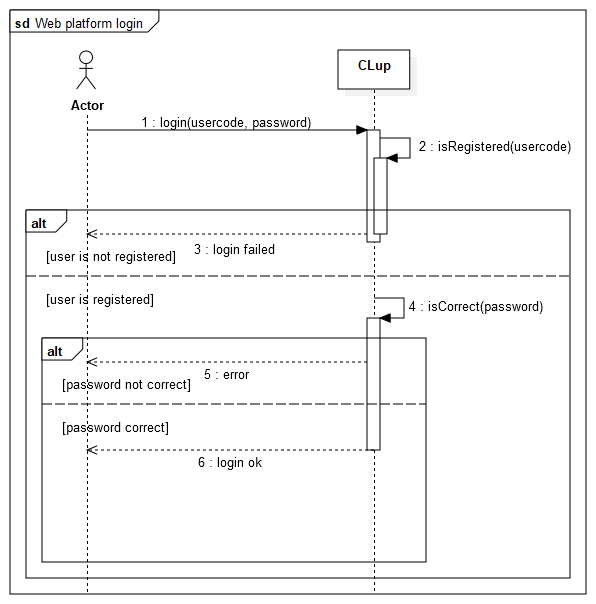
\includegraphics[width=\linewidth]{sd_web_platform_login}
		\caption{\textit{Web platform login} sequence diagram.}
	\end{figure}


	\begin{table}[H]
        \centering
        \begin{tabular}{@{}p{0.25\linewidth}p{0.71\linewidth}@{}}
            \toprule
            \textbf{Name} & Register new store \\

            \midrule
            \textbf{ID} & \usecaseindex{uc:registerStore} ~\\
            \midrule
            \textbf{Actors} & CLup admin \\
            \midrule
            \textbf{Entry conditions} &
            \begin{itemize}[leftmargin=.4cm,noitemsep,topsep=0pt,before=\vspace{-3mm},after=\vspace{-4mm}]
                \item The web platform is running.
                \item The CLup admin is logged in.
                \item The CLup admin has been contacted by a store manager.
            \end{itemize} \\
            \midrule
            \textbf{Flow of events} &
            \begin{enumerate}[label=\roman*.,leftmargin=.5cm,noitemsep,topsep=0pt,before=\vspace{-3mm},after=\vspace{-4mm}]
                \item The CLup admin goes to the "Add supermarket" page;
                \item The CLup admin fills in the form providing store information: name, address, PEC and timetables.
                \item The CLup admin submits the form.
                \item The system generates credentials for the store managers and store employee and send them  via email to the PEC address of the store.
            \end{enumerate} \\
            \midrule
            \textbf{Exit conditions} & The CLup admin has added a store to the platform. \\
            \midrule
            \textbf{Exceptions} &
            \begin{itemize}[leftmargin=.4cm,noitemsep,topsep=0pt,before=\vspace{-3mm},after=\vspace{-4mm}]
                \item If the store name is already used by another store, the system displays an error message asking the CLup admin to insert a different one.
            \end{itemize} \\

            \bottomrule
        \end{tabular}
        \caption{\textit{Register new store} use case description.}
    \end{table}

	\begin{figure}[H]
		\centering
		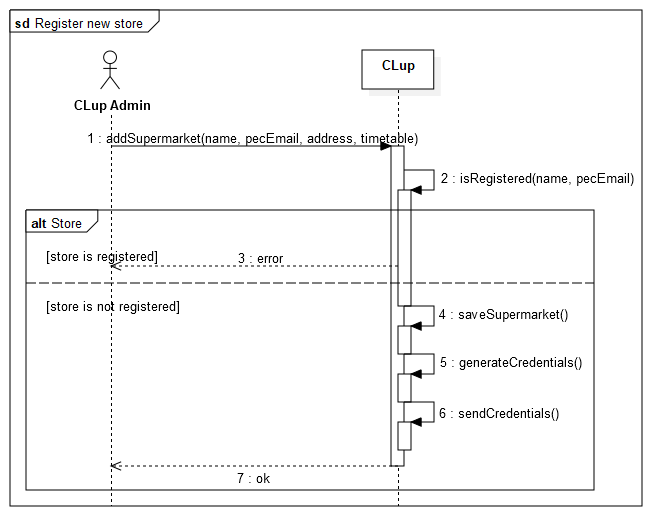
\includegraphics[width=\linewidth]{sd_register_new_store}
		\caption{\textit{Register new store} sequence diagram.}
	\end{figure}


	\begin{table}[H]
        \centering
        \begin{tabular}{@{}p{0.25\linewidth}p{0.71\linewidth}@{}}
            \toprule
            \textbf{Name} & Monitor bookings \\

            \midrule
            \textbf{ID} & \usecaseindex{uc:monitorBookings} ~\\
            \midrule
            \textbf{Actors} & Store manager \\
            \midrule
            \textbf{Entry conditions} &
            \begin{itemize}[leftmargin=.4cm,noitemsep,topsep=0pt,before=\vspace{-3mm},after=\vspace{-4mm}]
                \item The web platform is running.
                \item The store manager is logged in.
            \end{itemize} \\
            \midrule
            \textbf{Flow of events} &
            \begin{enumerate}[label=\roman*.,leftmargin=.5cm,noitemsep,topsep=0pt,before=\vspace{-3mm},after=\vspace{-4mm}]
                \item The Store manager go to the "Manage bookings list" page;
                \item The Store manager can filter bookings by date, time slot and categories;
                \item The system provides to the store manager a list with all the bookings that match the filter. If no filter are provided, a full list of all the bookings is shown.
            \end{enumerate} \\
            \midrule
            \textbf{Exit conditions} & The Store manager view the bookings. \\
            \midrule
            \textbf{Exceptions} &
            \begin{itemize}[leftmargin=.4cm,noitemsep,topsep=0pt,before=\vspace{-3mm},after=\vspace{-4mm}]
                \item If no bookings are available, an error is prompted to the store manager.
            \end{itemize} \\

            \bottomrule
        \end{tabular}
        \caption{\textit{Monitor bookings} use case description.}
    \end{table}

	\begin{figure}[H]
		\centering
		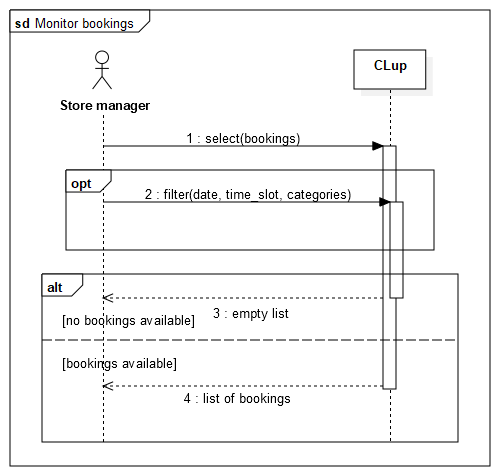
\includegraphics[width=\linewidth]{sd_monitor_bookings}
		\caption{\textit{Monitor bookings} sequence diagram.}
	\end{figure}


    \subsection{Traceability matrix}
    \begin{center}
        \begin{tabular}{@{}p{0.08\linewidth}cccccccccccccccccccccc@{}}
            \toprule
            \textbf{Item} &
            \clupref{req:custQueue} &
            \clupref{req:custTicket} &
            \clupref{req:custTicketKiosk} &
            \clupref{req:custNum} &
            \clupref{req:custTime} &
            \clupref{req:custGps} &
            \clupref{req:custLeave} &
            \clupref{req:custFilter} &
            \clupref{req:custTtl} &
            \clupref{req:custBook} &
            \clupref{req:custItems} &
            \clupref{req:custDelete} &
            \clupref{req:custNotifyDelete}\\
            \midrule

            \textbf{\prettyref{uc:retrieveTicket}} & \cmark & \cmark & & \cmark & \cmark & \cmark & & \cmark & \cmark \\
            \textbf{\prettyref{uc:bookVisit}} & \cmark & & & & & \cmark & & \cmark & \cmark & \cmark & \cmark \\
            \textbf{\prettyref{uc:deletePass}} & & & & & & & \cmark & \cmark & & & & \cmark & \cmark \\
            \textbf{\prettyref{uc:webLogin}} & \\
            \textbf{\prettyref{uc:registerStore}} & \\
            \textbf{\prettyref{uc:monitorBookings}} & \\
            \midrule
            \clupref{goal:custHazardSit} & \cmark & & & \cmark & \cmark & & & & \cmark & \cmark & \cmark \\
            \clupref{goal:storeHazardSit} & \\
            \clupref{goal:shortenTime} & \cmark & & & \cmark & \cmark & & & & \cmark & \cmark \\
            \clupref{goal:arriveOnTime} & \cmark & & & \cmark & \cmark & \cmark & & & \cmark & \cmark \\
            \clupref{goal:otherTasks} & \cmark & & & \cmark & \cmark & & & & \cmark & \cmark &\\
            \clupref{goal:easyExp} & & \cmark & & \cmark & \cmark & & \cmark & \cmark & & \cmark & & \cmark & \cmark \\
            \clupref{goal:enjoyService} & \cmark & & \cmark & & & & & & & \cmark \\
            \clupref{goal:monitorAccess} & \\
            \clupref{goal:knowInAdvance} & \\
            \clupref{goal:limitNumber} & \\

            \bottomrule
        \end{tabular}

        \begin{tabular}{@{}p{0.08\linewidth}cccccc|ccc|cc@{}}
            \toprule
            \textbf{Item} &
            \ref{req:mngLogin} &
            \ref{req:mngViewStore} &
            \ref{req:mngViewQueue} &
            \ref{req:mngViewBook} &
            \ref{req:mngCapStore} &
            \ref{req:mngDeleteTickets} &

            \ref{req:stfLogin} &
            \ref{req:stfViewStore} &
            \ref{req:stfViewQueue} &

            \ref{req:admRegister} &
            \ref{req:admCredentials}\\
            \midrule

            \textbf{UC.\ref{uc:retrieveTicket}} &&&&&&&&&&&\\
            \textbf{UC.\ref{uc:bookVisit}} &&&&&&&&&&&\\
            \textbf{UC.\ref{uc:deletePass}} &&&&&&&&&&&\\
            \textbf{UC.\ref{uc:webLogin}} & \cmark & & & & & & \cmark & & \cmark & \cmark \\
            \textbf{UC.\ref{uc:registerStore}} & & & & & & & & & & \cmark & \cmark \\
            \textbf{UC.\ref{uc:monitorBookings}} & \cmark & & & \cmark & & \cmark &&&&&\\
            \midrule
            \ref{goal:custHazardSit} &&&&&&&&&&&\\
            \ref{goal:storeHazardSit} & & \cmark & \cmark & \cmark & \cmark & \cmark & & \cmark & \cmark \\
            \ref{goal:shortenTime} &&&&&&&&&&&\\
            \ref{goal:arriveOnTime} &&&&&&&&&&&\\
            \ref{goal:otherTasks} &&&&&&&&&&&\\
            \ref{goal:easyExp} &&&&&&&&&&&\\
            \ref{goal:enjoyService} &&&&&&&&&&&\\
            \ref{goal:monitorAccess} & \cmark & \cmark & \cmark & \cmark & & & \cmark & \cmark & \cmark & \cmark & \cmark \\
            \ref{goal:knowInAdvance} & & \cmark & \cmark & \cmark & & & & \cmark & & & \\
            \ref{goal:limitNumber} & & & & & \cmark & \cmark & & & & \\

            \bottomrule
        \end{tabular}
    \end{center}

\section{Performance Requirements}
This section specifies numerical requirements placed on the software or on human interaction with the software as a whole.\newline
All the computation will take place on the servers of the system, therefore the mobile app shall be lightweight and occupy little memory on the customers' smartphones.
Since the majority of stores usually open only during daytime, the load in the night is expected to decrease considerably.
Regarding the scan process to let people enter or exit the store, at least 95\% of the passes scan shall be processed in less than 1 second: this is required in order to fulfil the goals of CLup.

\section{Design Constraints}

\subsection{Standards Compliance}
The system will store all the data in a database with the help of the DBMS. Indeed, the DBMS will provide a standard method to catalog, retrieve, and run queries on the data. Particular attention shall be reserved to the development of the modules interacting with the APIs of the DBMS.

Another relevant aspect is the API interface that CLup offers to the external services for scanning QR codes. The external service will communicate with the CLup servers via the REST API. By using a stateless protocol and standard operations, components can be managed and updated without affecting the system as a whole.\newline
It’s crucial to design REST APIs properly so that ease of use, security and performance will remain the core factors of the system.

\subsection{Other Constraints}
Regulatory policies have to be considered for the interaction between CLup and customers. The application, in fact, will ask the position of the customer while retrieving a ticket and while checking the queue status. Further information will be provided in the section \ref{req:privacy}.

\section{Software System Attributes}

\subsection{Reliability}
In order to guarantee continuity, services are required to be fault tolerant. Errors handling and fault containment mechanisms to prevent error propagation and data loss are to be arranged.

\subsection{Availability}
It is essential to have the lowest downtime possible, specially for the plain queue function (see section \clupref{desc:prodFunc}).
The ticketing components shall guarantee 99.9\% (\textit{three-nines}) of availability, so that only 8.76 hours of downtime per year are allowed.
Meanwhile the book-a-visit components shall guarantee 99\% (\textit{two-nines}) of availability, so that 3.65 days of downtime per year are allowed.

\subsection{Security}
The system shall perform role based access control (RBAC): an authorization scheme that grants access rights based on the role of the use. In particular, such components shall grant user authentication and authorization:
\begin{itemize}
    \item \textbf{Authentication}: request and verify the identity of CLup admin, store managers and employees attempting to login using a usercode and password.
    \item \textbf{Authorization}: verify the permissions of the logged user to perform any requested action (e.g. adding or removing a store, creating a new item category, etc.) before performing it.
\end{itemize}

\subsection{Maintainability}
The system shall be characterized by scalable and reusable modules which will be easier to maintain and replace in case of failure. Ordinary maintenance, for bug fixes and improvements, will be scheduled during night time, when the user traffic is minimal.\newline
The core aspects of maintainability and modularity will be addressed in the design document.

\subsection{Portability}
The web platform for store manager, staff and admin will be accessible by any web browser.\newline
The mobile application for customers must be accessible by as many users as possible, hence it must be developed for the major mobile OSes. Since the mobile app does not demand special functions, a non native approach can be adopted to fasten the development process.
The server side has no major requirements for portability.

\subsection{Usability}
The mobile app and the web platform of the system will be designed to be concise and user-friendly, with a graphical interface to help users identify the proper choice on the screen. It is expected that the 95\% of the users will be able to complete tasks without requiring assistance.

\section{Other Requirements}

\subsection{Privacy Requirements}\label{req:privacy}
The system shall ensure that the collection and transmission of personal data is handled in accordance with user’s expectation and regulations.\newline
In fact, to protect customers privacy, only the strictly necessary user data are requested to enjoy the app. Ensuring users privacy is protected positively influences user’s experience, acceptance and continuous use of the platform. For instance the system shall block unauthorized access to implicit information (e.g. location) and encrypt data transmission.

\subsection{Installation requirements}
For the system to work as intended, it shall be installed paired with an external solution which will carry out the scanning process of the QR codes for entering and exiting stores.\newline
The complete solution shall be installed in the specified environment (i.e. a store) within 4 working days.\newline
No specific installation requirements are necessary from the customer point of view. Indeed a customer may install the app right before starting to use it.
